\documentclass[12pt]{article}
\usepackage{geometry}                   
\usepackage{graphicx}
\usepackage{longtable}
\usepackage[latin1]{inputenc}
\usepackage{charter}
\usepackage{amssymb}
\usepackage[american]{babel}
\usepackage{epstopdf}
\DeclareGraphicsRule{.tif}{png}{.png}{`convert #1 `dirname #1`/`basename #1 .tif`.png}
\usepackage{natbib}
\bibpunct[]{(}{)}{,}{a}{}{,}
\bibliographystyle{linquiry2}
\usepackage[normalem]{ulem}
\setlength{\bibsep}{0ex}
\def\qroofpadding{0.2em}
\usepackage{stmaryrd}
\newcommand{\evaluation}[2][]{\ensuremath{\llbracket #2\rrbracket^{#1}}}
\usepackage{Sweave}
\usepackage{pgf}
\usepackage{tipa}
\usepackage{linguex}
\usepackage{tabularx}

\begin{document}

\title{Syntactic complexity from a cross-linguistic perspective: Relative clause extraposition in Russian}
\author{Dillon, Fedorenko, Levy}

\section{Introduction}
\label{sec:intro}

	In order to extract meaning from a sentence, it is necessary for comprehenders to recover the syntactic dependencies between the words in the sentence. Because the identification of syntactic relations is necessary for semantic interpretation, syntactic processing forms a crucial step in sentence comprehension. Theories of syntactic comprehension aim to provide an account of the mechanisms that allow the comprehender to extract syntactic structure from a string of words. Roughly speaking, these theories are built on two sources of evidence: evidence from the processing of ambiguous structures, and evidence from the processing of unambiguous, but complex, structures.
				
	The literature on processing relative clauses provides one example of an extremely fruitful line of research on syntactic complexity effects in unambiguous structures. In English, it is widely observed that object relative clauses (\ref{objextraction}) are more difficult to process than subject relative clauses (\ref{subjextraction}):
	
	\ex.	\label{rcs}
		\a.	\label{subjextraction} The reporter$_i$ that \_$_i$ attacked the senator admitted the error.
		\b.	\label{objextraction} The reporter$_i$ that the senator attacked \_$_i$ admitted the error. 
		
	The greater distance between the gap site (here marked by an underscore) in the object relative clause is associated with longer reading times (CITATIONS), increased activity in neurocognitive measures associated with linguistic processing (CITATIONS), and decreased accuracy in comprehension (CITATIONS). One class of theories accounts for the contrast in \ref{rcs} by appealing to the greater structural distance between the filler \textit{the reporter} and its gap site in ORCs (CITATIONS). Such \textit{structural complexity accounts} posit that the primary determinant of comprehension difficulty is the phrase-structural complexity of the dependencies, measured in terms of hierarchical distance (CITATIONS). A second class of accounts appeals to memory limitations to explain the difference between \ref{subjextraction} and \ref{objextraction}. These \textit{memory-based accounts} of this contrast hold that the need to maintain a filler in memory over a greater distance in the ORC configuration leads to difficulty (CITATIONS). Other variants of the memory-based account maintain that difficulty arises at the point of integration of the filler with its gap site, due to decay and / or interference from other constituents in memory (CITATIONS). Lastly, \textit{probabilistic expectations accounts} have proposed that the contrast between ORCs and SRCs reflects a difference in the likelihood of encountering an SRC versus an ORC in an unmarked situation (CITATIONS). 
	
	 A great deal has been learned through in-depth investigation of a small set of syntactic configurations in English. However, many researchers have noted that continued theory development requires a broader investigation into less widely investigated syntactic structures, as well as less-studied languages (CITATIONS). Perhaps most visibly, research into the processing of relative clauses has emphasized the need for a cross-linguistic approach. By comparing patterns of difficulty in comparable unambiguous structures across languages, it is sometimes possible to tease apart critical factors that may be confounded in any given language. For example, in English the linear and structural distance between the filler and the gap are confounded, making it difficult to determine which controls the complexity effects observed in examples like \ref{rcs} . However, in languages with prenominal relative clauses, linear and structural distance are dissociated. There are a number of studies that have investigated the prenominal analogs of \ref{rcs} in Mandarin Chinese (CITATIONS) and Korean (CITATIONS). On balance these studies appear to favor a structural account of the contrast between SRCs and ORCs (but c.f. CITATIONS). Likewise, in many languages, the structural complexity of a relative clause and the frequency of the RC structure are confounded. However, this is not true for Russian, where SRCs are not in general markedly more frequent than ORCs. In a study on processing relative clauses in Russian, Levy, Fedorenko and Gibson (CITATION) showed that in the absence of a clear frequency difference between SRC and ORC structures, Russian readers did not experience significant difficulty with the more syntactically complex ORC structures. 
	 
	Most work on syntactic complexity has focused on unbounded filler-gap dependencies where the filler precedes the gap, such as that see in English \textit{wh}-movement and relative clauses (see CITATIONS for an empirical overview). However, it is increasingly clear that a investigation into less well-studied syntactic dependencies will produce important insights into the nature of syntactic comprehension. For instance, Grant (CITATION) shows that comparative extraction shows an interestingly different pattern of difficulty from relative clause extraction, and a number of recent studies have looked at rightward movement constructions in English where the gap precedes the filler (CITATIONS).  In the present study we focus on this latter class of constructions. The present goal is to expand the empirical basis for theory development by presenting novel data on the processing of relative clause extraposition in Russian. 
	
	There is relatively little research on the comprehension of rightward movement, and many basic questions remain. Here we take up the question of how cross-linguistic variation impacts the processing difficulty that Levy and colleagues (CITATION) report for relative clause extraposition. The only existing experimental evidence that demonstrates processing difficulty for extraposed relative clauses comes from English. Because English is a language that relies overwhelmingly on word order cues to underlying syntactic structure (CITATIONS), one might question the generality of the results reported by Levy and colleagues. In the present study, we ask whether the complexity effects observed with extraposition extend to a language, Russian, where morphological cues to syntactic relations are weighted more highly than word order cues (CITATIONS). If English speakers encounter difficulty with extraposition simply because the discontinuous dependency requires them to rely on cues other than word order, then we do not expect the difficulty with extraposed relative clauses to extend to a language like Russian that relies relatively less on word order. On the other hand, if the processing difficulty associated with extraposition reflects core processes of syntactic prediction and memory search, then we expect the difficulty profile for extraposition to be relatively consistent across English and Russian. 
									
	\subsection{Processing rightward movement}
\label{sec:rightward}
	
	There are a number of constructions in English where it is possible to displace certain constituents rightwards from their canonical position in the sentence. Some examples are in \ref{rightmove}: 

	\ex.	\label{rightmove}
		\a.	\label{hnps} \textsc{heavy NP shift}: The senator attacked \_ yesterday [ the reporter who made an error ]
		\b.	\label{rcex} \textsc{RC extraposition}: The senator attacked a reporter \_  yesterday [ who made an error ]. 
		\c.	\label{ppex} \textsc{PP extraposition}: The senator attacked a reporter \_  yesterday [ from upstate New York's Adirondack region ]. 
		\d.	\label{compex} \textsc{clausal extraposition}: The senator said  \_ yesterday [ that the reporter made made an error ]. 
		\e.	\label{comparex} \textsc{comparative extraposition}: The senator attacked more reporters  \_ yesterday [ than I could even count ]. 

	The nature of the dependency between the gap in these sentences (marked by an underscore) and the filler that has been displaced to the right from that gap is a matter of active debate in theoretical syntax. One basic and unresolved question concerns the nature of the syntactic mechanism that links the gap with the rightward-displaced filler. It is not clear, for that matter, whether the constructions in \ref{rightmove} all rely on the same underlying syntactic mechanism (for discussion, see CITATIONS). There are three broad classes of syntactic mechanism that have been proposed for these structures. One proposal is that the relation between the gap and the filler uses the same mechanism as more familiar leftward movement seen in relative clause constructions and \textit{wh}-questions (CITATIONS). In the generative tradition this is implemented as a movement dependency (CITATIONS), and in non-transformational traditions this type of dependency is implemented through some mechanism of direct association, such as slash-passing mechanisms (CITATIONS).  Another possibility is that there is a special interpretive rule that links the displaced element and its original position in a manner similar to how pronouns achieve reference with their antecedents (CITATION). Lastly, certain mildly content-sensitive formalisms such as TAG and multiple CFGs hold that extraposition simply reflects a discontinuous constituent, and that the relationship of the extraposed constituent to its host is underlyingly the same as the dependency between any two daughters of a larger syntactic constituent (CITATIONS).  
	
	Although many questions remain concerning the appropriate syntactic treatment of these constructions, they all share a number of features that make them attractive objects of study from the point of view of online processing. For instance, they all present \textit{non-projective} or crossed syntactic dependencies. This is clearly visible in \ref{dep}, which gives a schematic view of the word-to-word dependencies in \ref{rcex} in the style of Dependency Grammar:
	
	   	\ex.	\label{rcex} \textsc{RC extraposition}: The senator attacked a reporter \_  yesterday  who made an error . (TO BE DRAWN)

	 Here it can be seen that the dependency between \textit{attacked} and \textit{yesterday} intersects the dependency between \textit{reporter} and \textit{who}. This type of crossed dependency is thought to be more complex than nested dependencies. This is reflected in e.g. the complexity of tabular parsing algorithms is significantly greater for grammars that allow for non-projective dependencies compared to those that do not (see CITATIONS; but note that it is not clear that this difficulty generally extends to incremental parsing algorithms c.f CITATION).
	 
	From the point of view of online filler-gap comprehension, rightward movement presents a number of interesting difficulties. Most obviously, the surface order of the filler and the gap are reversed from the filler-gap order seen in English \textit{wh}-movement and relative clause constructions. In addition, the gaps in \ref{rightmove} all contain examples of what what Fodor (CITATION) called a \textit{doubtful gap}: gaps whose existence may not be reliably inferred in an incremental parse of the string given the material that precedes the gap. In the absence of reliable cues to the presence of a gap in rightward movement dependencies, there arises the question of if and when the parser will actively predict a gapped analysis. Existing experimental evidence suggests that comprehenders will not generally posit a gap at the relevant point in examples like \ref{hnps} and \ref{rcex}. These findings stand in contrast to the processing of leftward filler-gap dependencies, where it is known that comprehenders will actively predict gaps even in positions where a gap is statistically very unlikely (CITATIONS). 
	
	Studies of rightward movement dependencies have shown that comprehenders incrementally posit a gap only under very limited conditions in examples like \ref{rightmove}. The exact conditions that allow comprehenders to predictively construct a gapped analysis are somewhat unclear. For instance, Staub, Clifton and Frazier (CITATION) investigated the processing of heavy noun phrase shift (HNPS), a syntactic alternation that involves shifting the object of a verb rightward over some intervening constituent. They found that the comprehender's willingness to adopt an HNPS analysis when she encounters a verb with a missing direct object is modulated by the strength of the transitivity bias of that verb. Comprehenders were shown to adopt an HNPS parse only when they encountered a verb that is obligatorily transitive, as in \ref{stauboblig}. For verbs that allowed both transitive and intransitive subcategorization frames (as in \ref{stauboptional}), comprehenders took a missing argument as a cue to an intransitive use of the verb, and did not project a HNPS analysis. This pattern suggests the comprehenders prioritize thematically complete analyses of partial input over those that contain missing arguments. This finding appears to suggest that a strong probabilistic bias for a gap following a verb is not enough to overcome a bias favoring maximal incremental interpretation. Staub and colleagues conclude that comprehenders only predict an HNPS analysis at the gap only when the grammar requires that there be a gap.

		\ex.	\label{hnpsstaub}
		\a.	\label{stauboblig} \textsc{obligatory gap}: Jack praised \_ from the stands [ his daughter's attempt to shoot a basket ].
		\b.	\label{stauboptional} \textsc{optional gap}: Jack watched \_ from the stands [ his daughter's attempt to shoot a basket ]. 

	Levy, Fedorenko, Breen and Gibson (CITATION) investigated the processing of relative clause extraposition in English. Across two self-paced reading experiments, they showed that processing an extraposed relative clause was associated with greater processing difficulty. This pattern of results was observed for extraposition from subject (\ref{levysubj}), as well as extraposition from object (\ref{levyobj}). 
	
			\ex.	\label{levysubj}
					\a.	 \textsc{in situ}: After the show, a performer who really impressed the audience came on and everyone went wild with applause.
					\b.	 \textsc{extraposed}: After the show, a performer \_ came on [ who really impressed the audience ] and everyone went wild with applause.

				\ex.	\label{levyobj}
					\a.	 \textsc{in situ}: The reporter interviewed the star about the movie which was filmed in the jungles of Vietnam.
					\b.	 \textsc{extraposed}: The reporter interviewed the star \_ about the movie [ who was filmed in the jungles of Vietnam ] .
	
	In both subject extraposition and extraposition from object cases, Levy and colleagues observed increased reading times in the relative clause region when it was extraposed compared to when it was in-situ. These results are compatible with those of Staub and colleagues, and they suggest that readers do not generally incrementally posit a gap of rightward movement. In the absence of a predicted dependency, additional processing is required to integrate the relative clause with its gap position, leading to the reading time slowdowns observed in Levy et al's Experiments 1 and 2. 

	Levy and colleagues further asked is comprehenders could utilize syntactic cues to incrementally posit a gap in examples like \ref{levyobj}. They manipulated the predictability of a relative clause postmodifier by contrasting NPs introduced by the definite determiner with those introduced by \textit{only those}. Both corpus and offline completion data suggested a strong preference for a relative clause postmodifier for \textit{only those} compared to \textit{the}. They predicted that this preference would lead comprehenders to anticipate a relative clause postmodifier, leading to eased processing of the extraposed relative clause. They tested this prediction by contrasting sentences like the following:
	
					\ex.	\label{levyonlythose}
					\a.	\textsc{weak expectation, in situ}: The chairman consulted the executives about the company which was acquired recently by an aggressive rival firm.
					\b.	\textsc{weak expectation, extraposed}: The chairman consulted the executives \_ about the company [ who was acquired recently by an aggressive rival firm ] .
					\c.	\textsc{weak expectation, in situ}: The chairman consulted only those executives about the company which was acquired recently by an aggressive rival firm.
					\d.	\textsc{weak expectation, extraposed}: The chairman consulted only those executives \_ about the company [ who was acquired recently by an aggressive rival firm ] .


	In conditions where the definite lead to a weak expectation for a post-modifier, they again observed a sizable reading time slowdown for extraposed relative clauses compared to their in-situ counterparts. However, when cued with \textit{only those}, there was no difference in reading times between in-situ and extraposed relative clauses. Like the results of Staub et al, this pattern shows that comprehenders can utilize strong predictive cues to infer the presence of a gap before the rightward-moved filler is encountered. The prediction of the dependency leads to faster processing. However, Levy and colleagues argued that comprehenders did not need to be forced to adopt a gapped analysis by their grammar; instead, graded probabilistic cues are sufficient to cause comprehenders to predict a gapped analysis.
	
	These results have the potential to be highly informative for debates about how comprehenders utilize grammatical information and probabilistic syntactic and semantic cues in constructing an incremental syntactic parse of the input. However, as described in the introduction, the empirical landscape for rightward gap-filler dependencies is currently quite limited. 
		
\subsection{Cues to syntactic dependencies in Russian}
	
	%Needs to be filled out. 
	
%%% All the primary analysis routines are in mainAnalysis.R



\section{Experiment}
\label{sec:experiment}

\subsection{Participants}
\label{sec:participants}

Seventeen native Russian speakers living in or visiting the United
States participated in this experiment at the University of California
at San Diego for cash compensation.  None had arrived in the United
States before age 13, and all reported that they continue to use
Russian on a regular basis and consider it the language they are most
comfortable with.
% 2.2.1. Materials

\subsection{Materials}
\label{sec:materials}


Twenty items (listed in full in the Appendix) were constructed following XXX
pattern.  Each participant saw only one of the four conditions of each
item according to a Latin square design.  These experimental stimuli
were interleaved with 32 items from an unrelated experiment and 52
random fillers such that no two experimental sentences were seen
consecutively.

%%% What were the comprehension questions like? One after every item? Did they require readers to resolve the RC attachment?


\subsection{Procedure}
\label{sec:procedure}


Sentences were presented to participants in a non-cumulative
word-by-word moving-window self-paced procedure on a PC laptop
computer running the Linger software \citep{rohde:lingermanual}. Each
trial began with a series of dashes displayed on the computer screen
in place of the words in the sentence. The first press of the space
bar revealed the first word in the sentence, and each subsequent press
of the space bar revealed the next word in the sentence and masked the
previous word. Punctuation was displayed together with the word
preceding it.  The times between button presses were recorded to the
nearest millisecond.  Each sentence was followed by a yes-or-no
comprehension question probing the participant's understanding of the
content of the sentence.  Written instructions in Russian were given
at the outset of the experiment.

\subsection{Data Analysis}
\label{sec:analysis}

Experimental sentences were divided into nine regions of interest as indicated in XXX. Raw reading times were analyzed independently within each region. Prior to analysis, RTs greater than 5000 ms or less than 100ms were excluded. After removing extreme outliers, RTs were further trimmed by removing observations that were more than three standard deviations from a condition mean within a given region. Trials that were incorrectly answered were not excluded from further analysis. This led to a rejection of 108 data points (3.5 \% of the data overall). Response time data were analyzed linear mixed effects (LME) models. The fixed effect structure of all LME models consisted of the experimental factors \textsc{structure}, \textsc{locality}, and their interaction, using simple difference coding (\textsc{structure}: -0.5 for VP attachment,  0.5 for NP attachment;  \textsc{locality}: 0.5 for local attachment, -0.5 for non-local attachment). All mixed effects models used participants and items as random effects, with random intercepts and slopes for all fixed effects (following \cite{barr2013}). In case the model with maximal random effects structure failed to converge, slopes for the interaction term were removed. Accuracy data were analyzed using mixed effects logistic regressions with identical fixed and random effect structure. \textit{p}-values were estimated from model \textit{t}-values by approximation to the standard normal distribution (\cite{baayen2008}).   
  
\subsection{Results}
\label{sec:results}

\subsubsection{Comprehension Accuracy}
\label{sec:acc}

Accuracy on comprehension questions was high, indicating that participants attended to the task. By condition accuracies are provided in \ref{acctable}. Logistic mixed effects modeling of the results indicate no significant differences between conditions. 

% latex table generated in R 3.0.1 by xtable 1.7-1 package
% Thu Oct  3 10:24:58 2013
\begin{table}[ht]
\centering
\begin{tabular}{rll}
  \hline
 & Local & Non-local \\ 
  \hline
NP & 0.94 (0.02) & 0.95 (0.03) \\ 
  VP & 0.96 (0.03) & 0.94 (0.03) \\ 
   \hline
\end{tabular}
\caption{Mean accuracy by condition for Experiment 1. By-participant standard errors in parentheses.} 
\end{table}
\subsubsection{Reading Times}
\label{sec:rts}

% latex table generated in R 3.0.1 by xtable 1.7-1 package
% Thu Oct  3 10:24:59 2013
\begin{table}[ht]
\centering
{\scriptsize
\begin{tabularx}{\textwidth}{rlllllllll}
  \hline
 & 1 & 2 & 3 & 4 & 5 & 6 & 7 & 8 & 9 \\ 
  \hline
1 & 637.5 (54) & 704.8 (74) & 856 (108) & 864.6 (93) & 718.6 (64) & 756.6 (59) & 583.6 (52) & 669.6 (53) & 975.9 (84) \\ 
  2 & 618.6 (48) & 725.8 (79) & 891.4 (105) & 861.4 (91) & 677.2 (59) & 721.5 (55) & 578.5 (33) & 667.5 (55) & 975.4 (82) \\ 
  3 & 663.4 (68) & 729.6 (73) & 870.1 (105) & 871.2 (77) & 701.4 (42) & 686.7 (58) & 566.3 (38) & 659.8 (51) & 935.8 (78) \\ 
  4 & 648.5 (62) & 735.1 (89) & 929.5 (130) & 915.1 (107) & 830.3 (80) & 951.4 (96) & 694.6 (58) & 622.9 (42) & 1136.4 (108) \\ 
   \hline
\end{tabularx}
}
\caption{Mean RTs in each region for Experiment 1. By-participant standard errors in parentheses.} 
\end{table}
Mean RTs in each region, along with by-participant standard error, is presented in \ref{rttable} and in \ref{rtfig}. Prior to the critical relative pronoun region, no significant effects of any experimental fixed effects were found. In the region immediately following the relative pronoun (region 6), mixed effects modeling showed a significant effect of \textsc{locality} ($\beta$ = -121 ($\pm$ 53), $p <$ 0.05), and a significant interaction of \textsc{locality} and \textsc{structure} ($\beta$ = 298 ($\pm$ 112), $p <$ 0.01). In region 7, there was a marginal effect of \textsc{locality} ($\beta$ = -62 ($\pm$ 34), $p <$ 0.1), as well as a marginal interaction \textsc{locality} and \textsc{structure} ($\beta$ = 129 ($\pm$ 66), $p <$ 0.1). Additionally, in region 9 there was a significant interaction of \textsc{locality} and \textsc{structure} ($\beta$ = 253 ($\pm$ 120), $p <$ 0.05), as well as a marginal effect of \textsc{locality} ($\beta$ = -127 ($\pm$ 77), $p <$ 0.1).

The critical interaction at region 6 was resolved by fitting a second LME model that used nested contrasts to estimate the effect of \textsc{locality} within each level of the \textsc{structure} factor. The results of this model indicate a significant effect of locality for VP attachment conditions ($\beta$ = -270 ($\pm$ 91), $p <$ 0.01). There was no significant effect of locality for NP attachment conditions ($\beta$ = 28 ($\pm$ 61), $p =$ 0.646).


\begin{figure}
\begin{center}
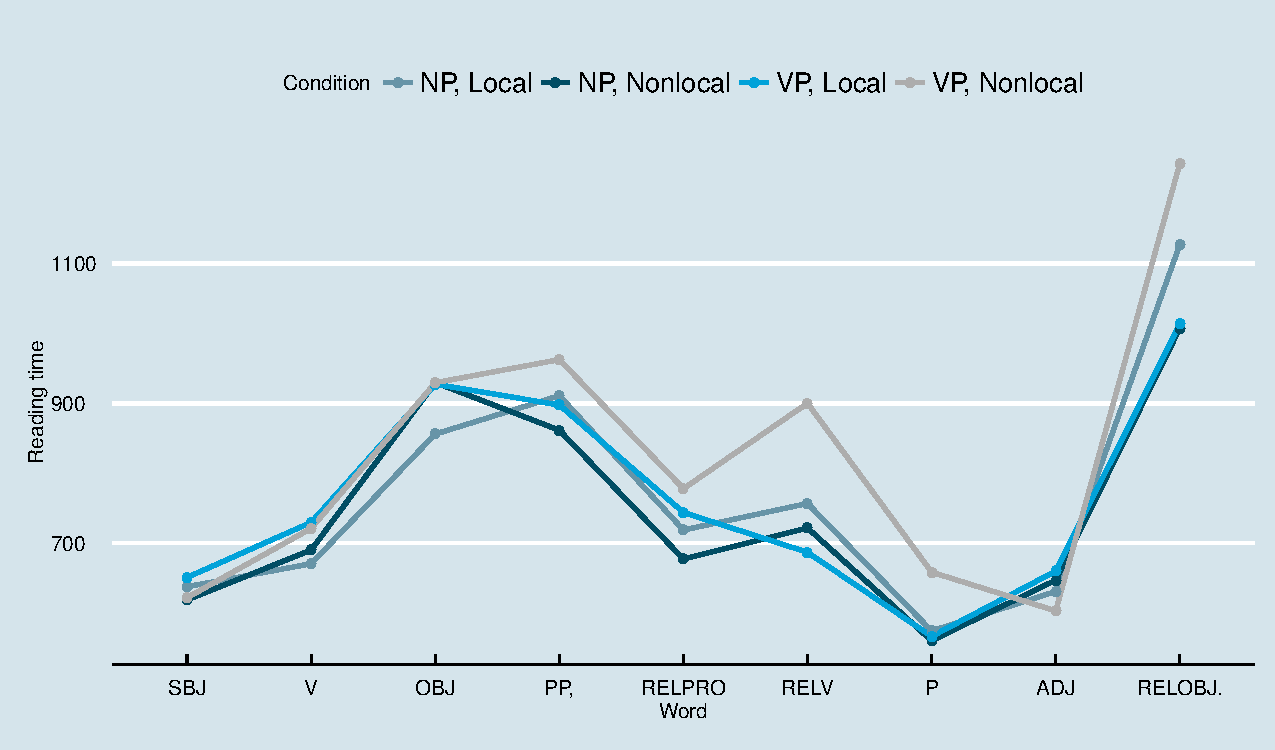
\includegraphics{russian-extraposed-rcs-mainplot}
\end{center}
\caption{Mean reading times in Experiment 1. Error bars represent standard error by participants.}
\label{rtfig}
\end{figure}


\section{Discussion}
\label{sec:experiment}

\subsection{Summary of results}

	%% Compare to size of effect in Levy et al Expt 2

\bibliographystyle{apalike}
\bibliography{russian-extraposed-rcs}

\appendix
\section{Experimental materials}




\end{document}

%%% Local Variables: 
%%% mode: latex
%%% TeX-master: t
%%% End: 
